%
% zweidimensionale.tex
%
% (c) 2020 Prof Dr Andreas Müller, Hochschule Rapperswil
%
\subsection{Zweidimensionale Signale
\label{subsection:qam:zweidimensional}}
Wir suchen also nach einem Verfahren, mit welchem wir nicht nur
ein einzelnes zeitabhängiges Signal $I(t)$ übertragen können, sondern
auch noch ein zweites Signal, welches wir mehr oder weniger aus
historischen Gründen $Q(t)$ nennen wollen\footnote{Das Signal $I(t)$
heisst auch die In-phase-Komponente und $Q(t)$ Quadratur-Komponente}.
Man kann sich die beiden Signale zum Beispiel also die beiden
Stereokanäle eines Audiosignals vorstellen.
Wir stellen uns die beiden Komponenten als untrennbar zusammengehörig
vor, es ist daher sinnvoll, sie als zweidimensionalen Vektor
\[
\vec{v}(t)
=
\begin{pmatrix}I(t)\\Q(t)\end{pmatrix}
\]
zu schreiben.
Dieser Vektor beschreibt zu jeder Zeit $t$ einen Punkt in der
$I$-$Q$-Ebene.
Zu verschiedenen Zeiten beschreibt $\vec{v}(t)$ eine Kurve
in der Ebene.
Mit einem Oszilloskop im X-Y-Modus kann man den Vektor
sichtbar machen.
Zum Beispiel führt das Signal
\begin{equation}
I(t) = \cos t,\quad
Q(t) = \sin 3t
\qquad
\Rightarrow
\qquad
\vec{v}(t)
=
\begin{pmatrix}
\cos t\\
\sin 3t
\end{pmatrix}
\label{eqn:qam:liss1}
\end{equation}
auf die in Abbildung~\ref{figure:qam:lissajous} dargestellte Kurve.
\begin{figure}
\centering
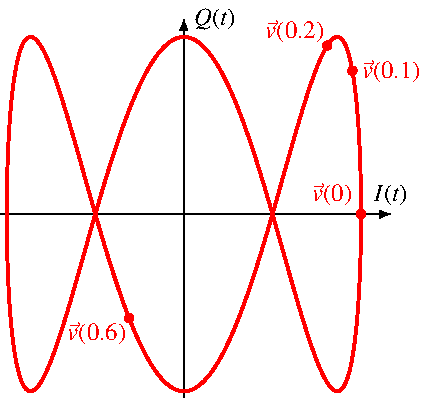
\includegraphics[width=0.48\hsize]{applications/qam/lissajous.pdf}
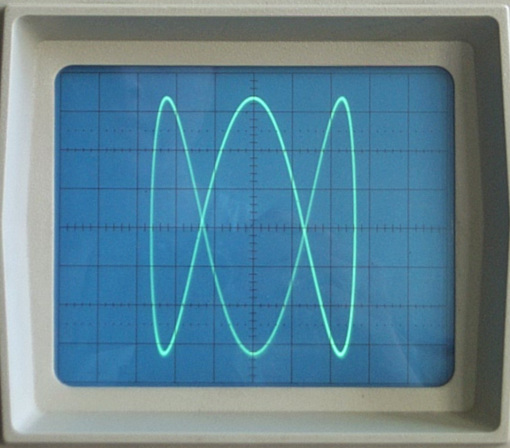
\includegraphics[width=0.48\hsize]{applications/qam/lissajous.jpg}
\caption{Lissajous-Figur des zweidimensionalen Signals
\eqref{eqn:qam:liss1} kann auf einem Oszilloskop im X-Y-Modus
sichtbar gemacht werden.
\label{figure:qam:lissajous}}
\end{figure}
Solche Kurven sind bekannt als Lissajous-Figuren.
Mit komplizierteren Funktion $I(t)$ und $Q(t)$ kann fast jede
Linienzeichnung auf den Schirm des Oszilloskops gezaubert werden,
wie zum Beispiel auch die Internet ``Kunstform'' der Oscilloscope
Music (\url{https://www.youtube.com/watch?v=qnL40CbuodU}) zeigt.
In Abbildung~\ref{figure:qam:pilze} werden zum Beispiel Pilze und
ein Schmetterling mit zwei geeigneten Funktionen $I(t)$ und $Q(t)$
gezeichnet.

\begin{figure}
\centering
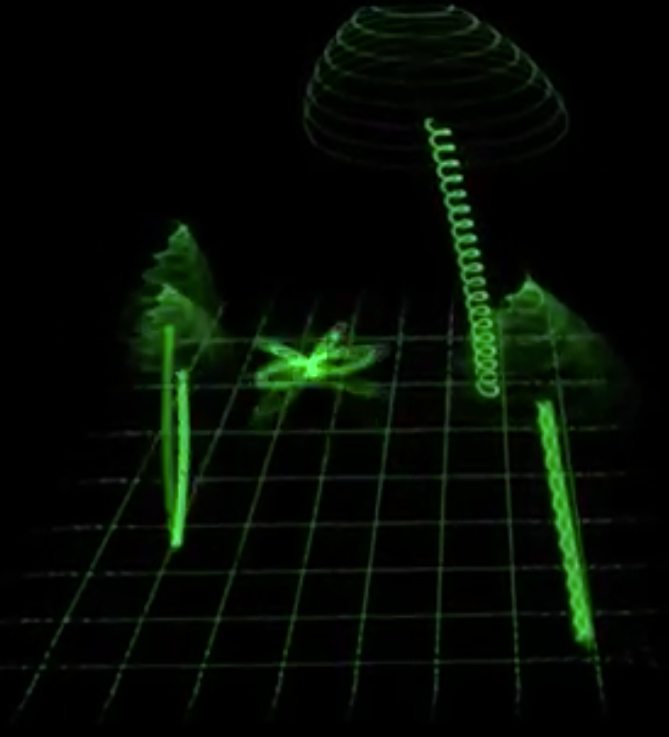
\includegraphics[width=0.5\hsize]{applications/qam/pilze.png}
\caption{Pilze und ein Schmetterling gezeichnet von zwei Signalen
$I(t)$ und $Q(t)$ aus dem Video \url{https://youtu.be/rtR63-ecUNo}
\label{figure:qam:pilze}}
\end{figure}



